\section{Sensor block}
This section describes in detail how the sensor block handles the the output of the Hall effect sensors and sends it to the comparator block.

\subsection{Description}
The responsibility of the sensor block is to handle the output from the Hall effect sensors and determine the position of both the pan part and the tilt part of the system. The controller block rely on this information and thus this block form the basis of the control method chosen.

\subsection{Theory}
Hall effect sensors are sensors that change their voltage output based on proximity of a magnetic field. If combined with the right circuitry it can be used a switch, giving a digital output. When placed around the rotating axis of a motor with the right relative distance, the Hall effect sensors can be used determine the position, direction, rotational velocity and the position of the axis.
There is a disc on the axis of the motor. It is divided into 6 sections, alternating between two levels of magnetization. Around the magnet, two Hall effect sensors are placed at an angle of slightly less than 90 degrees(See figure \ref{Motor_magnet}). As the motor axis rotate, the magnetized parts move past the sensors and the magnetic field, they are subjected to, changes. Because the Hall effect sensor is a little “off” the output will have an overlap, see figure \ref{Hallcounteksemple}. This is what is used to determine the direction.

\begin{figure}[h!]
  \centering
  \begin{minipage}[b]{0.6\textwidth}
    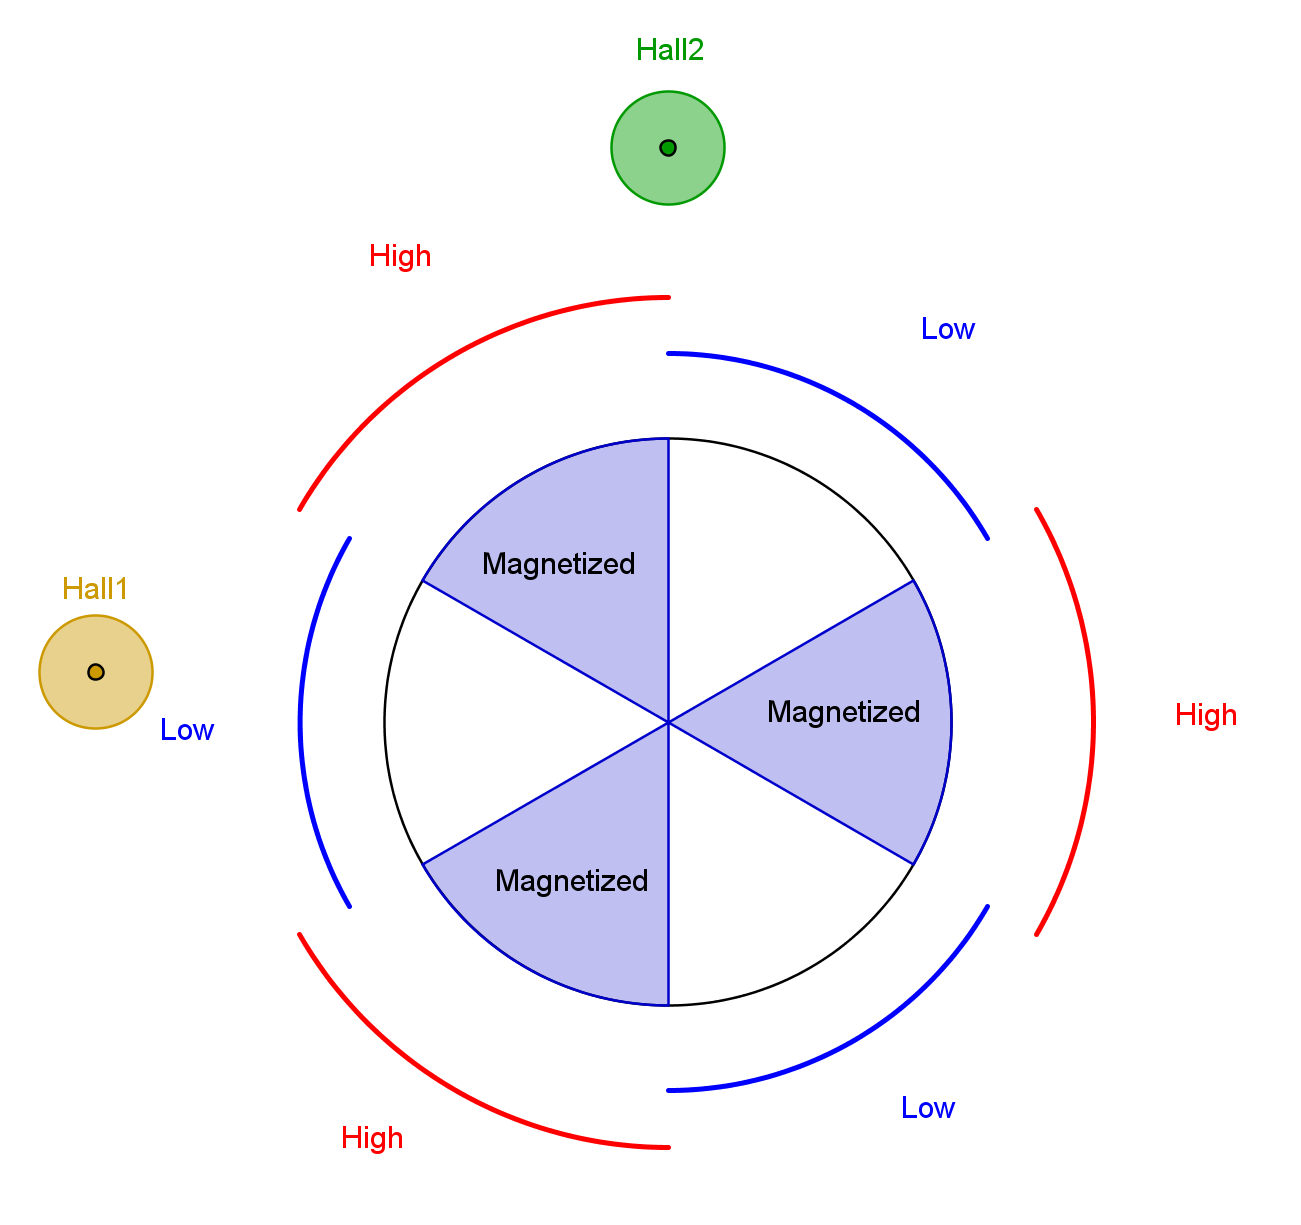
\includegraphics[width=\textwidth]{Billeder/FPGA/Motor_Magnets.png}
    \caption{This is an example of how the Hall effect sensors is placed around the disk.}
    \label{Motor_magnet}
  \end{minipage}
  \hfill
  \begin{minipage}[b]{0.3\textwidth}
    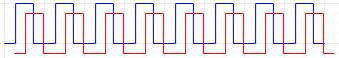
\includegraphics[width=\textwidth]{Billeder/FPGA/Hallcounteksemple.PNG}
    \caption{As the axis rotates, the output changes}
    \label{Hallcounteksemple}
  \end{minipage}
\end{figure}

\subsection{Implementation}

The Hall counter is the sensor block.
Every time the Hall effect sensors gives an output the Hall counter is updated. There are 1080 “tachs” or changes in the output of the Hall effect sensor, for one revolution. To be able to move both clockwise and counterclockwise, the starting position i set to half of the total: 540.
This i done to avoid working with negative values, as that can contribute to unnecessary difficulty in the implementation.

It starts out with sampling the value of the sensors. The value of the sensor is read and shifted into a vector of two bits as seen in figure \ref{fig:Shift code pos}

\begin{figure}[h!]
\centering
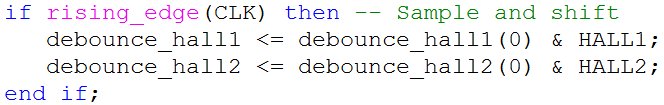
\includegraphics[scale=0.5]{Billeder/FPGA/Shift_code_example.png}
\caption{ An example of how the the value is sampled and shifted }
\label{fig:Shift code pos}
\end{figure}


If no change have been registered, the position doesn't change and a new sample is taken. As seen in figure \ref{fig:Pos_change_flowchart}. If a change is detected then a series of “if statements” determines whether the change in position is positive or negative.

\begin{figure}[h!]
\centering
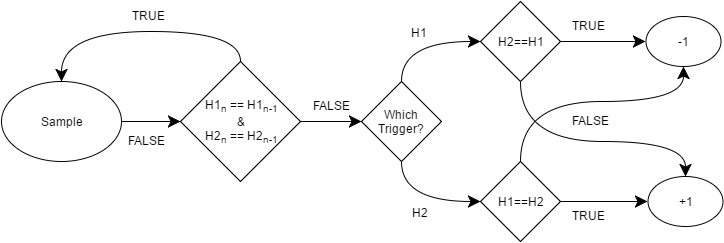
\includegraphics[scale=0.5]{Billeder/FPGA/Pos_change_flowchart.png}
\caption{ Flowchart of how the position changes in relation to different Hall effect sensor outputs }
\label{fig:Pos_change_flowchart}
\end{figure}

A small example of the of the code involved can be seen in figure \ref{fig:Pos_change_code_example}

\begin{figure}[h!]
\centering
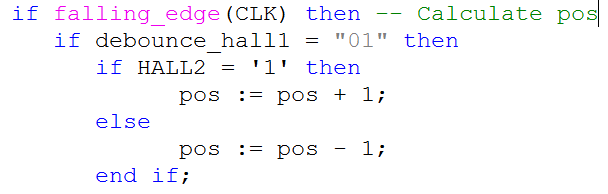
\includegraphics[scale=0.5]{Billeder/FPGA/Calculate_pos_code_example.png}
\caption{ Small bit of code that shows how the position is calculated based on the Hall effect sensor output }
\label{fig:Pos_change_code_example}
\end{figure}

\subsection{Test}
To make sure the code behaves in the intended way a test bench have been made. It simulates the codes response to changing output from the Hall effect sensors. The first two bars show the Hall effect sensors and their changing values. The next bar is the clock and under that one the position.

As can be seen in figure \ref{fig:Pos_change_testbench}, the position is steadily decreasing in value.
If the position reaches the max value (108010 or 00000100001110002) the position is set to 0. If the position reaches -1 it is set to the max value minus one.

\begin{figure}[h!]
\centering
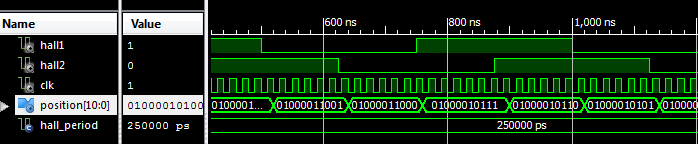
\includegraphics[scale=0.8]{Billeder/FPGA/Pos_change_testbench.png}
\caption{ Testbench of how the position changes based on Hall effect sensor outputs }
\label{fig:Pos_change_testbench}
\end{figure}

\subsection{Discussion}
As there is only two Hall effect sensors and the max rate of change in their output is a lot less than the possible sampling rate, it is fairly easy to calculate the change in position of the motor. However having only two sensors and only 6 different magnetization levels limits the accuracy of the measurements. If the axis of the motor moves in the area between a rising or falling edge but never reaching one on either sensors the change in position cannot be measured. More sensors would give a higher precision but also require more calculations in order to determine whether the change is positive or negative.
One more error that can be experienced is if the axis end up in a position where one of the sensors is “stuck” on a rising or falling edge. If that happens the position will constantly flip between the two values.
Lastly as magnets are used they sometimes “stick” to a certain position.
All this combined with the slack in the belt transferring the rotation from the motor to either the pan or tilt and the small distance before the teeth of the belt and gear meshes, this limits the overall precision of the system

\subsection{Conclusion}

The component works as expected and sends the current position of the system to the comparator block.